\chapter{Spécifications fonctionnelles}

\section{Spécifications générales}

\subsection{Aspect général du projet}

Le projet se découpe en quatre grandes parties qui sont :
\begin{itemize}
	\item la préparation des données ;
	\item le stockage des données dans une BDD ;
	\item l'interface avec le reconnaisseur ;
	\item l'IHM.
\end{itemize}

\paragraph{}
Ces parties sont résumées sur le schéma 1, déjà abordé dans le rapport de
pré-étude.

\paragraph{}
\begin{mdframed}[frametitle={Figure 1 : Décomposition du projet (mode apprentissage)}, innerbottommargin=10]
\begin{center}
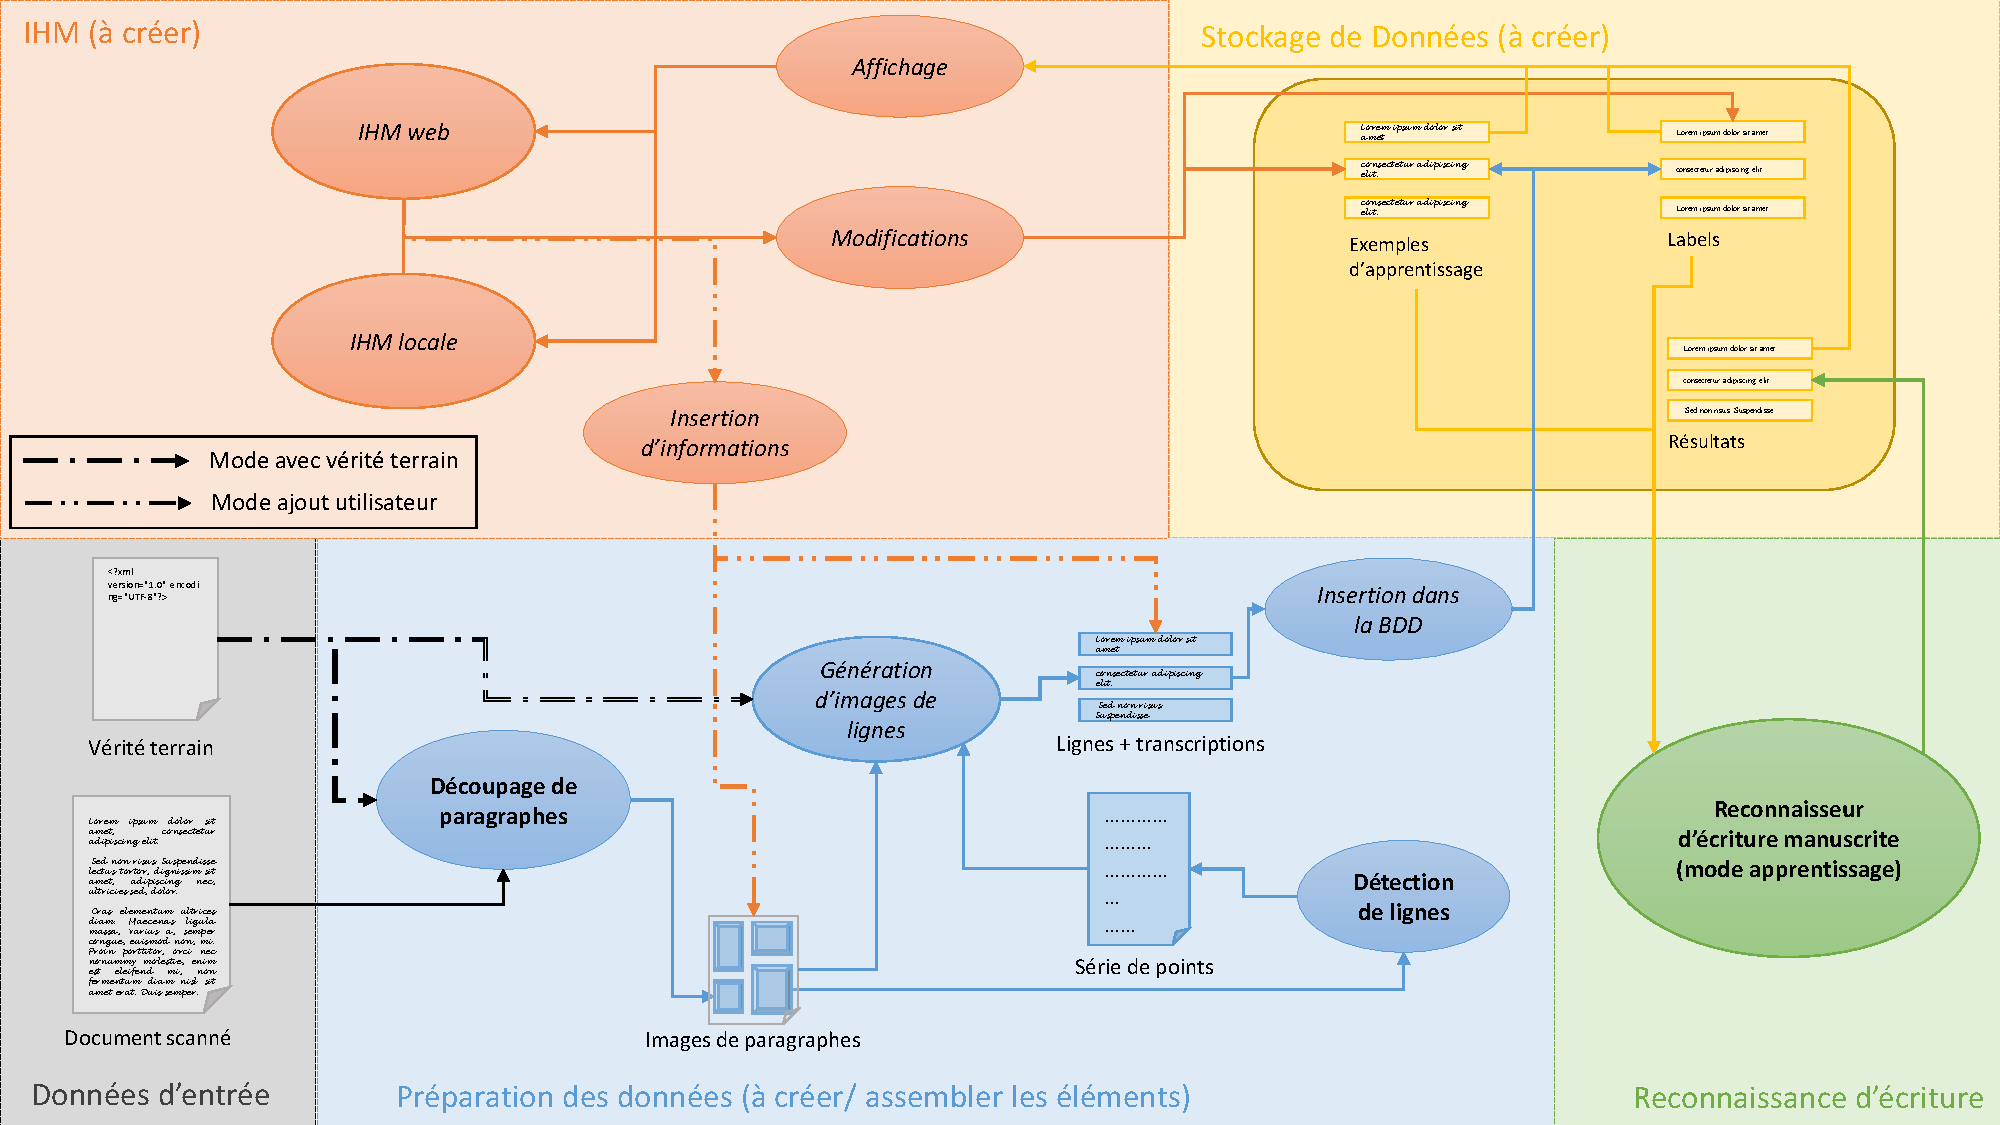
\includegraphics[width=\linewidth]{schema_mode1.1.pdf}
\end{center}
\end{mdframed}

\paragraph{}
Le projet se présente sous la forme d’un programme, principalement écrit en
\href{http://scala-lang.org}{Scala}. En effet, lors du précédent rapport,
nous avions déjà évoqué ce choix personnel, qui permet de travailler à la
fois avec un langage fonctionnel et avec la JVM. Par la suite tous les éléments
décrits seront donc considérés comme écrits en Scala, et pour toute exception,
le langage utilisé sera précisé.

\paragraph{}
La partie découpe de documents prend en entrée des documents scannés contenant
de l’écriture manuscrite, en extrait les informations contenues sous la forme
de couples imagette-transcription et les stocke dans la BDD. Le
\textit{framework} de gestion de bases de données utilisé est codé en Java.
Les langages Scala et Java étant interopérables, car tournant tous deux sur la
JVM, notre code Scala est donc compatible avec ce \textit{framework}. Le code
de notre logiciel concernant la base de données sera écrit en Java.

\paragraph{}
Ces informations stockées sont mises à disposition d’un classifieur, pour qu’il
puisse apprendre dessus. Ce classifieur ne fait pas partie du cadre de
l’application, mais vient se greffer à celle-ci. Le programme doit donc faire
en sorte que les données de la BDD puissent être accessibles par le classifieur.
Le classifieur n’étant pas intégré au programme, il peut être changé à tout
moment. L’application doit néanmoins pouvoir le faire fonctionner en 3 modes :
apprentissage, évaluation et production. Les données stockées dans la base sont
ainsi divisées en sous-ensembles, chacun correspondant à un mode de
fonctionnement.

\paragraph{}
Le tout est géré par l’utilisateur grâce à une interface Web, en JavaScript
pour une plus grande accessibilité et une meilleure portabilité. Ce choix a
également pour but de faciliter l’évolution de l’application vers une solution
multi-utilisateurs distants, où plusieurs personnes s‘y connecteraient via
Internet. Chaque partie sera expliquée plus en détails dans la suite du rapport.

\subsection{Côté utilisateur}

Le logiciel à créer fonctionnera donc suivant plusieurs modes de fonctionnement :
\begin{itemize}
	\item apprentissage ;
	\item évaluation ;
	\item production.
\end{itemize}

\paragraph{}
Les trois modes ne sont pas à implémenter avec la même priorité, seul le mode
apprentissage est nécessaire pour obtenir un résultat fonctionnel. Les deux
modes suivants sont à implémenter suivant le temps restant.

\paragraph{}
Le mode apprentissage a pour objectif de faire apprendre un système de
reconnaissance d’écriture. Le logiciel génère une base d’apprentissage pour un
système de reconnaissance d’écriture manuscrite et fournit les données
produites en entrée du reconnaisseur. Celui-ci peut alors les utiliser pour
apprendre à retranscrire correctement du texte.

\paragraph{}
Du point de vue de l'utilisateur du logiciel, par l’intermédiaire de l’IHM, il
peut :
\begin{enumerate}
\item charger un document dans la base de données, accompagné d’une vérité
terrain ;
\item charger un document dans la base sans vérité terrain ;
\item annoter ledit document pour lui associer une nouvelle transcription ;
\item lancer l’apprentissage du système de reconnaissance ;
\item modifier les données contenues dans la base :
\begin{enumerate}
\item supprimer un document ;
\item déplacer un document vers un autre sous-ensemble ;
\end{enumerate}
\item changer de mode de fonctionnement.
\end{enumerate}

\newpage

\begin{mdframed}[frametitle={Figure 2 : Diagramme de cas d'utilisation (mode apprentissage)}, innerbottommargin=10]
\begin{center}
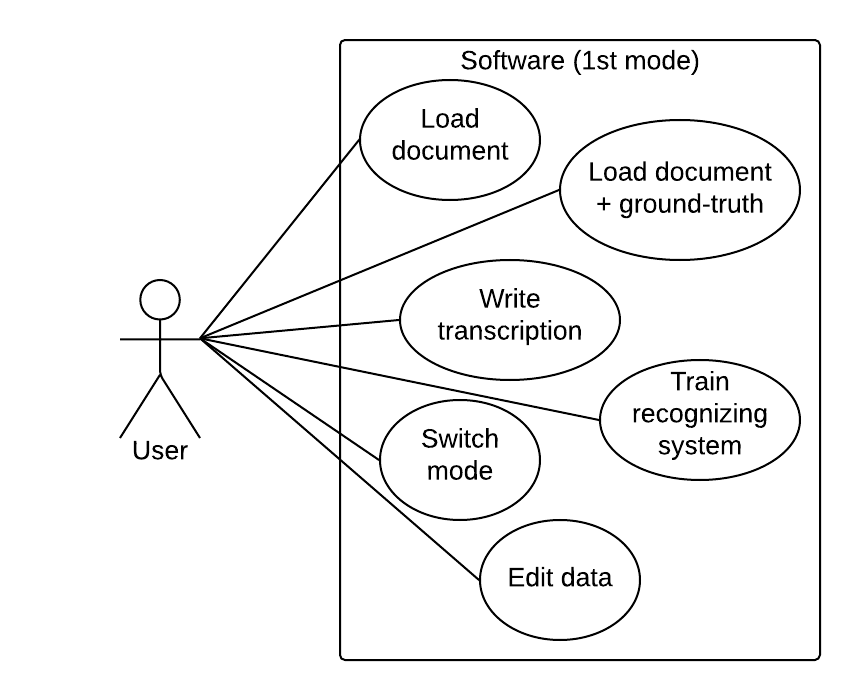
\includegraphics[scale=0.6]{Usecase_1.png}
\end{center}
\end{mdframed}

\paragraph{}

Le mode évaluation a pour objectif d’évaluer un système de reconnaissance. Ce
mode est en général utilisé après avoir effectué un apprentissage avec le
reconnaisseur. Il permet de vérifier l’efficacité de l’apprentissage effectué.

\paragraph{}

Dans ce mode, toujours par l’intermédiaire de l’IHM, l’utilisateur peut :
\begin{enumerate}
\item charger un document, accompagné d’une vérité terrain (la vérité terrain
est obligatoire dans ce mode de fonctionnement, pour que l’évaluation soit
correcte) ;
\item lancer l’évaluation du système de reconnaissance ;
\item modifier les données contenues dans la base :
\begin{enumerate}
\item supprimer un document ;
\item déplacer un document vers un autre sous-ensemble ;
\end{enumerate}
\item changer de mode de fonctionnement.
\end{enumerate}

\paragraph{}

\begin{mdframed}[frametitle={Figure 3 : Diagramme de cas d'utilisation (mode évaluation)}, innerbottommargin=10]
\begin{center}
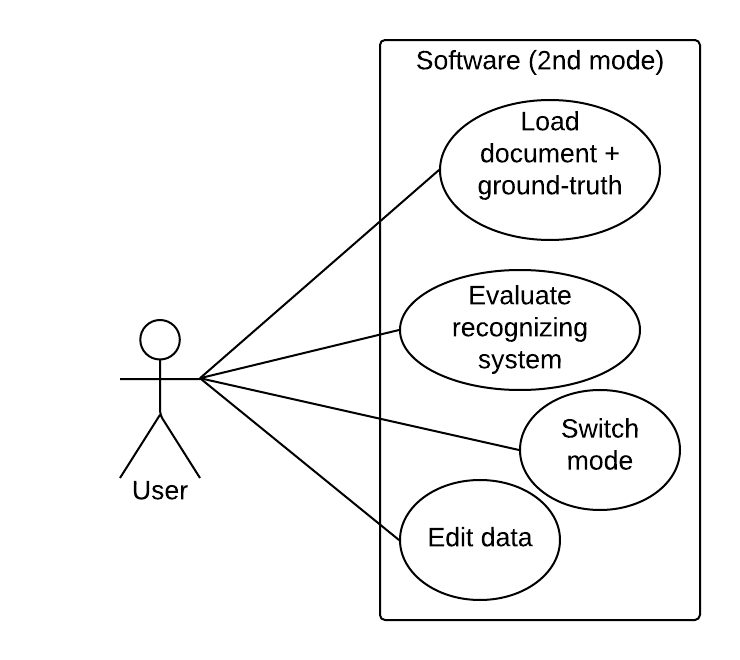
\includegraphics[scale=0.6]{Usecase_2.png}
\end{center}
\end{mdframed}

\paragraph{}
Le mode production a pour objectif d’utiliser un système de reconnaissance afin
d’obtenir une transcription pour des documents n’en ayant pas. Ce mode est en
général utilisé sur un reconnaisseur entraîné, dont l’apprentissage a été
évalué, et ayant donc obtenu de bons résultats. Il s’agit également d’un mode
de démonstration, permettant d’utiliser le reconnaisseur de manière ludique.
Il pourra être utilisé lors de la démonstration de fin de projet.

\paragraph{}
Dans ce mode, via l'intermédiaire de l’IHM, l’utilisateur peut :
\begin{enumerate}
\item charger un document sans vérité terrain ;
\item écrire une transcription manuellement, pour compléter ou corriger la
transcription du reconnaisseur ;
\item jouer à des mini-jeux en utilisant le reconnaisseur (le contenu des
mini-jeux n’a pas encore été établi, cette option étant annexe au projet) ;
\item modifier les données contenues dans la base :
\begin{enumerate}
\item supprimer un document ;
\item déplacer un document vers un autre sous-ensemble ;
\end{enumerate}
\item changer de mode de fonctionnement.
\end{enumerate}

\paragraph{}
\begin{mdframed}[frametitle={Figure 4 : Diagramme de cas d'utilisation (mode production)}, innerbottommargin=10]
\begin{center}
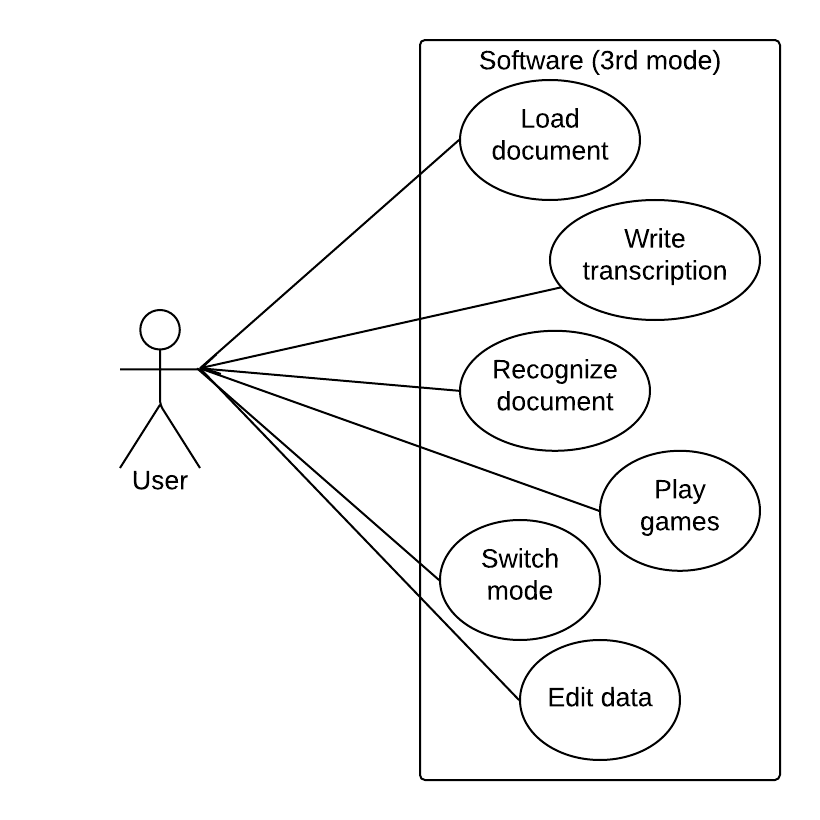
\includegraphics[scale=0.6]{Usecase_3.png}
\end{center}
\end{mdframed}

\paragraph{}
Le logiciel ne possède pas de système de reconnaissance d’écriture intégré.
Cette partie, comme précisé précédemment, y est simplement greffée. Il n’est
pas prévu de pouvoir changer de reconnaisseur via l’interface graphique, cette
opération étant rare et pouvant même ne jamais avoir lieu au cours de la vie du
logiciel. Néanmoins, il doit être possible pour un développeur de système de
reconnaissance d’écriture manuscrite utilisant notre logiciel de changer le
reconnaisseur. Cette possibilité sera donc incluse dans le projet.

\paragraph{}
\begin{mdframed}[frametitle={Figure 5 : Diagramme de cas d'utilisation (pour développeur)}, innerbottommargin=10]
\begin{center}
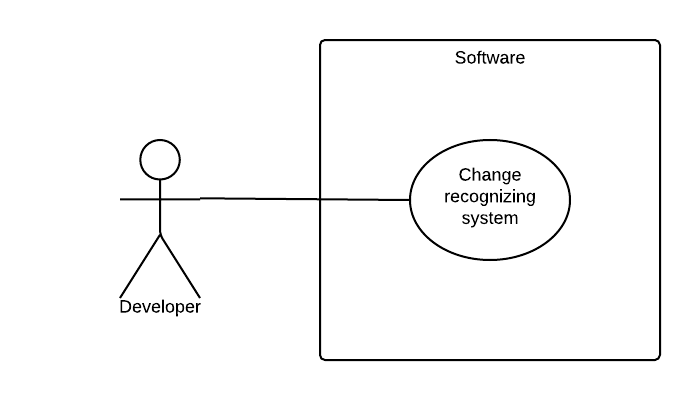
\includegraphics[scale=0.7]{Usecase_Dev.png}
\end{center}
\end{mdframed}